We now consider an elastic solid with square section of dimension $l=3m$ in the ($\vect{e}_1,\vect{e}_2$) plane, infinite in direction $\vect{e}_3$ so that the plane strain assumption holds (\textit{i.e. $\eps_{33}=\eps_{13}=\eps_{23}=0$}). The solid suddenly undergoes a tensile load on a part of its left boundary (see figure \ref{fig:2D_planeStrain}\subref{subfig:2D_problem}) leading to shear and pressure waves propagating in the medium until reflection on the right end.
\begin{figure}[h!]
  \centering
  \subcaptionbox{Geometry and boundary conditions\label{subfig:2D_problem}}{\begin{tikzpicture}[scale=0.9]
  \draw[thick] (0,0) --(3,0)--(3,3)--(0,3)--(0,0);
  \foreach \x in {0.5,1.,...,2.5} 
  \draw(\x,-0.2)circle(0.2);
  \foreach \x in {0.25,0.75,...,2.75} 
  \draw(3.2,\x)circle(0.2);
  \draw(0,-0.4)--(3.,-0.4);
  \draw(3.4,0)--(3.4,3);
  \fill [pattern=north east lines](0.0,-0.8)rectangle+(3,0.4);
  \fill [pattern=north east lines](3.4,0.)rectangle+(0.4,3);
  \draw[>=stealth,<->](0,3.1)--node[above=1pt]{\footnotesize $l=3 \: m$}(3,3.1);
  \draw[>=stealth,<->](0.1,0)--node[right=1pt]{\footnotesize $a=1 \: m$}(0.1,1);
  \foreach \x in {0.,0.25,...,1} 
  \draw[>=stealth,<-] (-0.5,\x)--(0.,\x);
  \node(a)at(-1.75,0.5){\footnotesize $\tens{\sigma}\cdot\vect{e}_1=\matrice{\sigma^d\\0 \\0}$}; 
  \draw[>=stealth,->](-1.5,2)--(-0.5,2)node(a)[anchor=north]{\footnotesize $\vect{e}_1$};
  \draw[>=stealth,->](-1.5,2)--(-1.5,3)node(a)[anchor=south]{\footnotesize $\vect{e}_2$};
\end{tikzpicture}


%%% Local Variables:
%%% mode: latex
%%% TeX-master: "../../mainManuscript"
%%% End:
} \qquad
  \subcaptionbox{Material points set and grids \label{subfig:2d_meshes}}{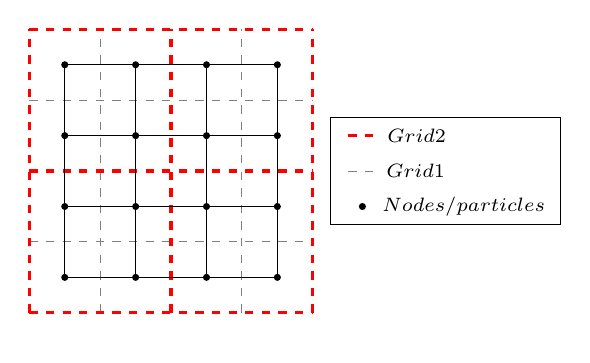
\begin{tikzpicture}[scale=0.9]
  \draw (0,0) --(3,0)--(3,3)--(0,3)--(0,0);
  \draw[white] (0.,0) -- (0,-0.8);
  %%% Grid 1
  \foreach \y in {-0.5,0.5,...,3.5} 
  \draw[dashed,gray] (-0.5,\y) -- (3.5,\y);
  \foreach \x in {-0.5,0.5,...,3.5} 
  \draw[dashed,gray] (\x,-0.5) -- (\x,3.5);
  %%% Grid 2
  \foreach \y in {-0.5,1.5,...,3.5} 
  \draw[dashed,Red,very thick] (-0.5,\y) -- (3.5,\y);
  \foreach \x in {-0.5,1.5,...,3.5} 
  \draw[dashed,Red,very thick] (\x,-0.5) -- (\x,3.5);
  \foreach \y in {0.,1.,...,3.} 
  \foreach \x in {0.,1.,...,3.} 
  \fill (\x,\y) circle(0.05);
  \foreach \y in {0.,1.,...,3.} 
  \draw (0,\y) -- (3.,\y);
  \foreach \x in {0.,1.,...,3.} 
  \draw (\x,0) -- (\x,3);
  \draw (3.75,0.75) rectangle (7.,2.25);
  \fill (4.2,1.) circle (0.05) node [right] {\scriptsize$ \: \: \text{Nodes / particles}$};
  \draw[dashed,gray] (4.,1.5) -- (4.4,1.5) node [right] {\scriptsize$\color{black} \text{Grid 1}$};
  \draw[dashed,very thick,Red] (4.,2.) -- (4.4,2.) node [right] {\scriptsize$\color{black} \text{Grid 2}$};
\end{tikzpicture}


%%% Local Variables:
%%% mode: latex
%%% TeX-master: "../manuscript"
%%% End:
}
  \caption{Geometry, loading and boundary conditions for the tensile impact problem on a two-dimensional elastic medium.}
  \label{fig:2D_planeStrain}
\end{figure}
The MPM and the DGMPM are compared to a $Q1$ finite element (bilinear approximation) solution coupled with a central difference explicit time integrator, computed with the code Cast3M \cite{Castem}.
Since an upper bound of the CFL number cannot be determined for the DGMPM scheme using RK2 time discretization for two-dimensional problems, we consider the DGMPM-Euler scheme in the remainder of the manuscript.
More specifically, the following simulations have been carried out by means of the CTU method.

The domain is discretized such that material points are equivalent to finite element nodes: $l\times l \equiv 28 \times 28$ particles and nodes. Moreover, two arbitrary grids are used for the DGMPM so that either one or four material points lie in every cells according to the situations depicted in figure \ref{fig:2D_planeStrain}\subref{subfig:2d_meshes}.
Figure \ref{fig:2delast_comparison} shows the isovalues of the longitudinal stress $\sigma_{11}$ in the two-dimensional medium at two different times with the traction force set to $\sigma^d=200\: Mpa$.
The two instants at which the solutions are depicted correspond to incident and reflected waves. In addition, the stress profiles along the bottom boundary of the domain are plotted in figures \ref{fig:elastlines}\subref{subfig:line_elast1} and \ref{fig:elastlines}\subref{subfig:line_elast2} for the same times.

Analogously to one-dimensional problems, the figures show that DGMPM solutions do not suffer from spurious oscillations while FEM and MPM one exhibits numerical noise.
\begin{figure}[h!]
  \centering
  \begin{tikzpicture}
  \begin{groupplot}[group style={group size=4 by 2,
      ylabels at=edge left, yticklabels at=edge left,
      horizontal sep=1.ex,
      vertical sep=2ex,},
    enlargelimits=0,
    xmin=0.,xmax=1., ymin=-0.,ymax=1.
    ,axis on top,scale only axis,xtick=\empty,ytick=\empty,width=0.2\linewidth,
    colorbar style={
      title style={
        font=\scriptsize,
        at={(1,.25)},
        anchor=north west
      },yticklabel style={font=\scriptsize}
      ,at={(current axis.south east)},anchor=south west
    }]
    %% FIRST ROW (time 1 = 3.5e-4s)
    %%% RANGE -2.0e7 -- 2.9e8
    \nextgroupplot[ylabel={$t=3.5\times 10^{-4} \:s$},title={(a) FEM}]\addplot graphics[xmin=0.,xmax=1., ymin=-0.,ymax=1.] {chapter4/pngFigures/fem_stress_115.png};
    \nextgroupplot[title={(b) DGMPM 1ppc}]\addplot graphics[xmin=-0.,xmax=1., ymin=-0.,ymax=1.] {chapter4/pngFigures/dgmpm1ppc_stress_115.png};
    \nextgroupplot[title={(c) DGMPM 4ppc}]\addplot graphics[xmin=-0.,xmax=1., ymin=-0.,ymax=1.] {chapter4/pngFigures/dgmpm4ppc_stress_115.png};
    \nextgroupplot[title={(d) MPM 1ppc},
    colorbar,colorbar style={
      title= {$\sigma_{11}\: (MPa)$},
      ytick={-5.7e-2,2.e-1,2.9e-1},
      yticklabels={-57,200,290},
    }]
    \addplot[scatter,scatter src=y,mark size=0.pt] coordinates {(0.,-5.7e-2) (0.,2.9e-1)};% Fake extreme values to fix scale
    \addplot graphics[xmin=-0.,xmax=1., ymin=-0.,ymax=1.] {chapter4/pngFigures/mpm_stress_115.png};

    %% SECOND ROW (time 2 =1.e-3s)
    %%% RANGE -4.4e7 -- 4.2e8
    \nextgroupplot[ylabel={$t=1.0\times 10^{-3} \:s$}]\addplot graphics[xmin=0.,xmax=1., ymin=-0.,ymax=1.] {chapter4/pngFigures/fem_stress_338.png};
    \nextgroupplot[]\addplot graphics[xmin=-0.,xmax=1., ymin=-0.,ymax=1.] {chapter4/pngFigures/dgmpm1ppc_stress_338.png};
    \nextgroupplot[]\addplot graphics[xmin=-0.,xmax=1., ymin=-0.,ymax=1.] {chapter4/pngFigures/dgmpm4ppc_stress_338.png};
    \nextgroupplot[colorbar,colorbar style={
      title= {$\sigma_{11}\: (MPa)$},
      ytick={-4.3e-2,2.e-1,4.8e-1},
      yticklabels={-43,200,480},
    }]
    \addplot[scatter,scatter src=y,mark size=0.pt] coordinates {(0.,-4.3e-2) (0.,4.8e-1)};% Fake extreme values to fix scale
    \addplot graphics[xmin=-0.,xmax=1., ymin=-0.,ymax=1.] {chapter4/pngFigures/mpm_stress_338.png};
    
  \end{groupplot}
\end{tikzpicture}



%%% Local Variables:
%%% mode: latex
%%% TeX-master: "../mainManuscript"
%%% End:

  \caption{Isovalues of longitudinal stress $\sigma_{11}$ solution of the tensile impact problem in a two-dimensional elastic medium. Comparison between FEM (CFL=0.9), DGMPM-CTU using 1ppc (CFL=1) or 4ppc (CFL=0.23), and MPM using 1ppc (CFL=0.7).}
  \label{fig:2delast_comparison}
\end{figure}
The decrease in the CFL number involved by 4ppc yields a less accurate resolution of the jump discontinuity carried by the longitudinal pressure wave than for 1ppc, which captures the incident right-going discontinuity (see figure \ref{fig:elastlines}\subref{subfig:line_elast1}).
Next, the interaction of shear and pressure waves traveling in the medium leads to a curved stress profile upstream of the discontinuity that is captured differently by all methods.  
\begin{figure}[h!]
  {\phantomsubcaption \label{subfig:line_elast1}}
  {\phantomsubcaption \label{subfig:line_elast2}}
  \begin{tikzpicture}
  \begin{groupplot}[group style={group size=2 by 1,
ylabels at=edge left, yticklabels at=edge left,horizontal sep=3.ex,
xticklabels at=edge bottom,xlabels at=edge bottom},
ymajorgrids=true,xmajorgrids=true,ylabel=$\sigma_{12} \: (Pa)$,
axis on top,scale only axis,width=0.4\linewidth, every x tick scale label/.style={at={(xticklabel* cs:1.05,0.75cm)},anchor=near yticklabel},ymin=-0.5e6,ymax=.5e9]
\nextgroupplot[ylabel=$\sigma_{11} (Pa)$,xlabel=$x (m)$]
\addplot[Red,very thick,no markers] table[x=Points:0,y=S11] {chapter4/csvFiles/2delast_fem_115.csv};
\addplot[Blue,very thick,mark=+,only marks,mark size=3pt] table[x=Points:0,y=stress_11] {chapter4/csvFiles/2delast_ctu1ppc_115.csv};
\addplot[Purple,very thick,mark=square*,only marks] table[x=Points:0,y=stress_11] {chapter4/csvFiles/2delast_ctu4ppc_115.csv};
\addplot[Orange,very thick,mark=x,only marks,mark size=3pt] table[x=Points:0,y=mpm_S11] {chapter4/csvFiles/2delast_mpm_115.csv};

\nextgroupplot[legend style={at={($(0.12,-0.35)+(0.9cm,1cm)$)},legend columns=2},xlabel=$x (m)$]
\addplot[Red,very thick,no markers] table[x=Points:0,y=S11] {chapter4/csvFiles/2delast_fem_338.csv};
\addplot[Blue,very thick,mark=+,only marks,mark size=3pt] table[x=Points:0,y=stress_11] {chapter4/csvFiles/2delast_ctu1ppc_338.csv};
\addplot[Purple,very thick,mark=square*,only marks] table[x=Points:0,y=stress_11] {chapter4/csvFiles/2delast_ctu4ppc_338.csv};
\addplot[Orange,very thick,mark=x,only marks,mark size=3pt] table[x=Points:0,y=mpm_S11] {chapter4/csvFiles/2delast_mpm_338.csv};
\addlegendentry{fem}
\addlegendentry{ctu 1ppc}
\addlegendentry{ctu 4ppc}
\addlegendentry{mpm}
   
  \end{groupplot}
\end{tikzpicture}


%%% Local Variables:
%%% mode: latex
%%% TeX-master: "../../mainManuscript"
%%% End:




































%%% Local Variables:
%%% mode: latex
%%% TeX-master: "../../mainManuscript"
%%% End:

  \caption{Evolution of longitudinal stress $\sigma_{11}$ along the bottom boundary of the elastic square plate. Comparison between FEM (CFL=0.9), DGMPM-CTU using 1ppc (CFL=1) or 4ppc (CFL=0.23), and MPM using 1ppc (CFL=0.7).}
  \label{fig:elastlines}
\end{figure}
On the other hand, the cylindrical profile of the longitudinal stress is quite well described by FEM and DGMPM with 1ppc, even after reflection of the fixed boundary as can be seen in figure \ref{fig:2delast_comparison}. The smoothness of DGMPM solutions using 4ppc and the oscillations in MPM results however prevent to distinguish this structure.

Figure \ref{fig:elastlines}\subref{subfig:line_elast2} also shows that the stress level on the right boundary of the domain differs from one method to another. Furthermore, MPM and FEM solutions after the passage of the reflected waves oscillate a lot compared to these of DGMPM schemes. In particular, the stress levels greatly differ after the reflection of the pressure wave.


%%% Local Variables:
%%% mode: latex
%%% TeX-master: "../mainManuscript"
%%% End:
